
\section{Eseguire A-CLus Esteso}


Per avviare la versione estesa del progetto A-CLus, è necessario seguire i seguenti passaggi:
\begin{enumerate}
    \item Accedere alla directory \texttt{A-CLUS\_Esteso/Jar + Bat}
    \item All'interno della suddetta cartella, eseguire il file \texttt{Start Server.bat} con doppio click, mantenendo attiva la finestra del prompt dei comandi
    \item Procedere con l'avvio del file \texttt{Start Client.bat} tramite doppio click, il quale genererà un'ulteriore finestra di comando
    \item Aprire Telegram e cercare "A-CLus" utilizzando il tag "@A\_Clus\_bot" oppure cliccando sul \href{https://shorturl.at/r07hj}{link diretto}
\end{enumerate}

\begin{tcolorbox}[colback=white, colframe=gray, title=Avvertenza]
    È necessario mantenere attivi i terminali del server e del client per garantire la comunicazione tra tutte le componenti del sistema.
\end{tcolorbox}

\subsection{Avvio dall'ambiente di sviluppo}

La procedura di avvio del progetto A-CLus può essere eseguita anche direttamente dall'ambiente di sviluppo, in maniera analoga alla versione base. 

\begin{enumerate}
    \item Aprire il progetto \texttt{A-CLus\_Esteso}
    \item Eseguire il file \texttt{MultiServer.java} presente nella cartella \texttt{server/src/server} per avviare il server
    \item Eseguire il file \texttt{Main.java} presente nella cartella \texttt{client/src/client} per avviare il client
    \item Aprire Telegram e cercare "A-CLus" utilizzando il tag "@A\_Clus\_bot" oppure cliccando sul \href{https://shorturl.at/r07hj}{link diretto} per accedere al bot 
\end{enumerate}

\subsection{Guida operativa al bot Telegram}

Una volta assicurati che il server e il client siano in esecuzione, è possibile interagire con il bot Telegram.


\begin{figure}[h!]
    \centering
    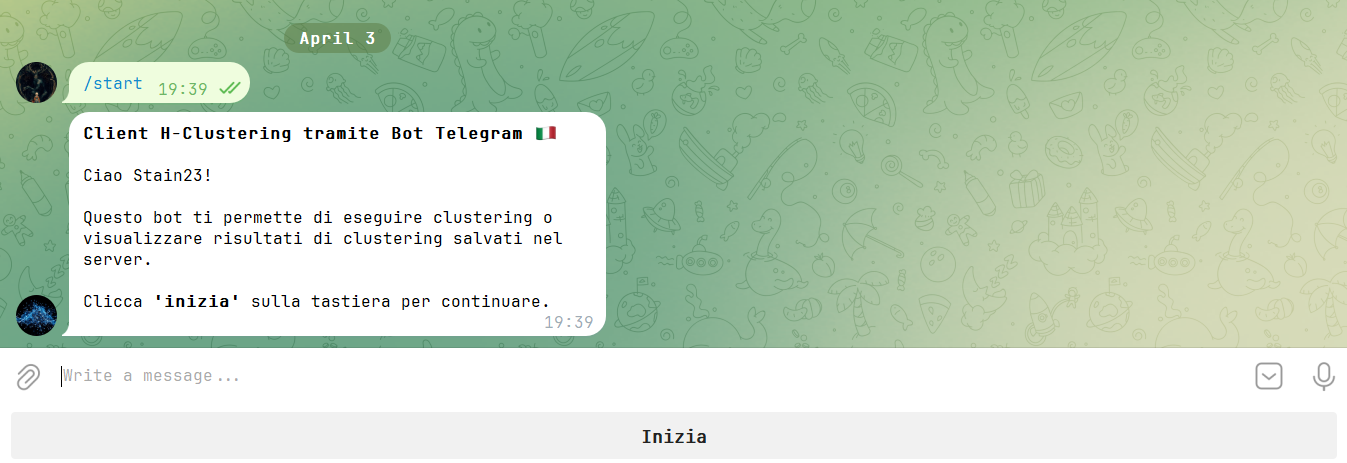
\includegraphics[width=.5\textwidth]{images/tg iniziale.png}
    \caption{Interfaccia iniziale del bot Telegram}
\end{figure}

La schermata iniziale del bot si presenta con un messaggio di benvenuto. È possibile sia scrivere \texttt{/inizia} che cliccare sul bottone per cominciare l'interazione con il bot.

\begin{figure}[h!]
    \centering
    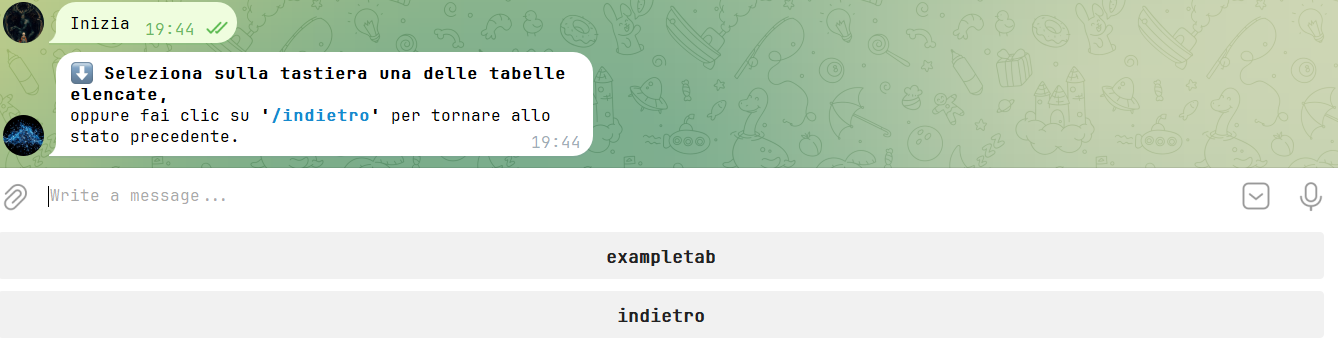
\includegraphics[width=.5\textwidth]{images/inizia tg.png}
    \caption{Interfaccia di scelta del database}
\end{figure}

Una volta iniziata l'interazione, verrà chiesto all'utente di selezionare il database da cui prendere i dati. In alternativa, si può schiacciare il bottone indietro per termianre l'interazione. 

\begin{figure}[h!]
    \centering
    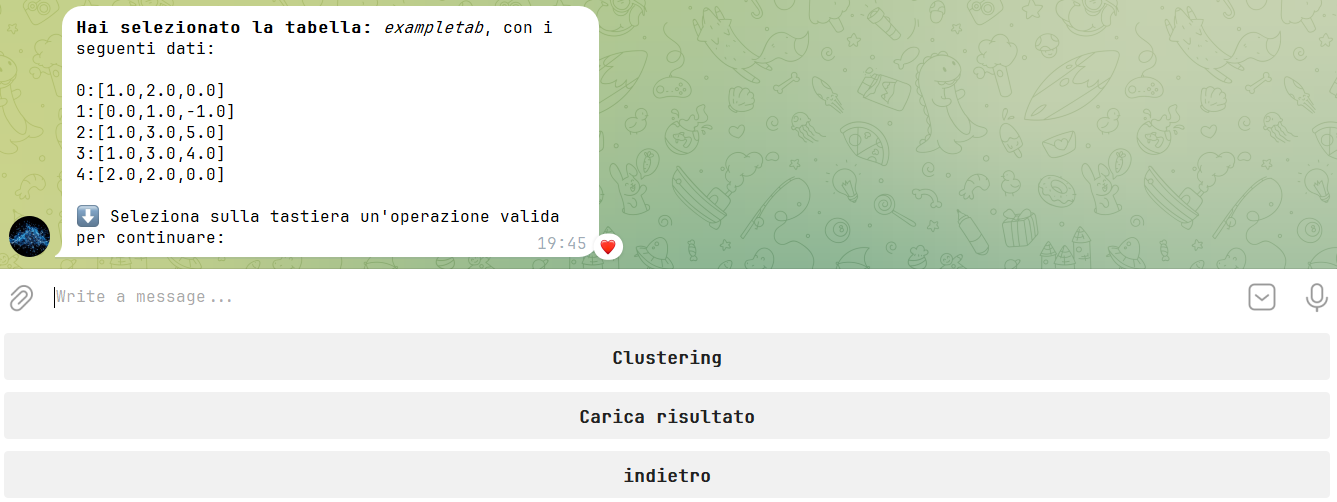
\includegraphics[width=.5\textwidth]{images/tg schemrata clustering.png}
    \caption{Selezione dell'azione da eseguire}
\end{figure}

Una votla scelto il database, sarà possibile scegliere l'azione da eseguire. In questo caso, si può scegliere di eseguire un clustering nuovo, oppure di caricare un dendrogramma precedentemente salvato. In alternativa, si può schiacciare il bottone indietro per tornare alla schermata di selezione del database.

Nel caso si scelga di caricare un risurisultato  precedentemente calcolato, il bot chiederà di inserire il nome del file con cui è stato salvato, e restituirà il dendrogramma contenuto nel file. 

Nel caso, invece, che si scelga di eseguire un nuovo clustering, il bot chiederà informazioni  riguardo la profondità del dendrogramma da calcolare, e il metodo di calcolo delle distanze da utilizzare.

\begin{figure}[h!]
    \centering
    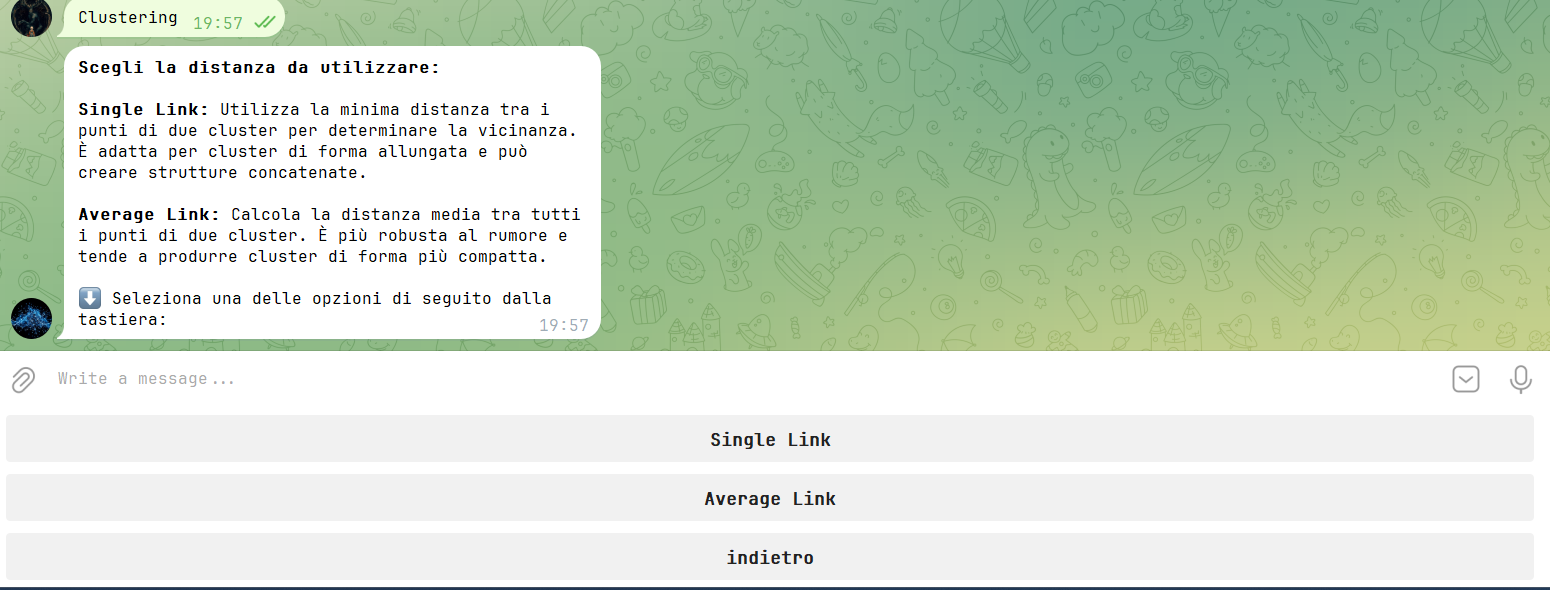
\includegraphics[width=.5\textwidth]{images/distanza da calcaolare tg.png}
    \includegraphics[width=.5\textwidth]{images/profondità tg.png}
    \caption{Informazioni per il calcolo del dendrogramma}

\end{figure}

Una volta inseriti i dati, il bot calcolerà il dendrogramma in base ad essi, e chiederà se si vuole salvare il dendrogramma in un file. Di seguito, chiederà di inserire il nome del file in cui salvare il dendrogramma.


\begin{figure}[h!]
    \centering
    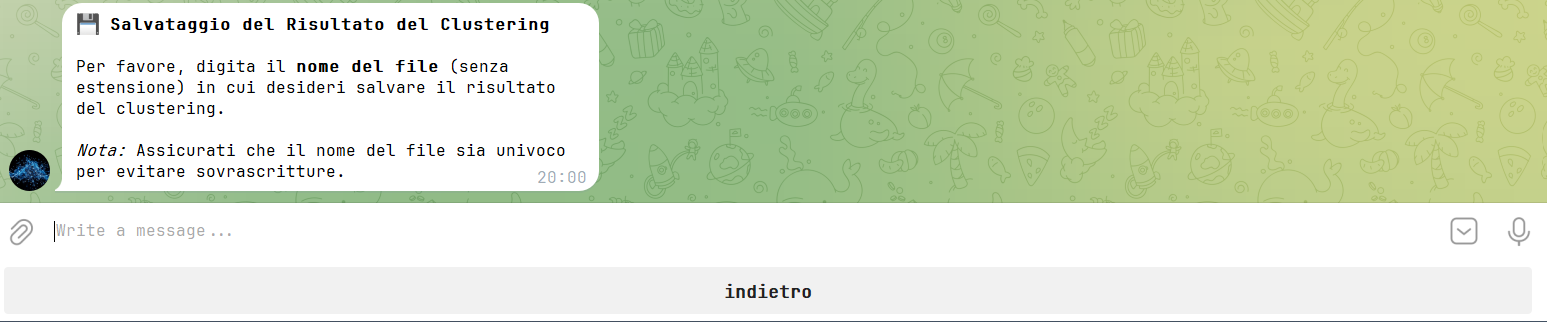
\includegraphics[width=.5\textwidth]{images/finale tg.png}
    \caption{Schermata finale}
\end{figure}


\subsection{Test A-CLUS ESTESO}

Durante la fase di testing della versione estesa, sono stati verificati i seguenti scenari:

\begin{itemize}
    \item \textbf{Resilienza della connessione Telegram:} 
    Il sistema gestisce correttamente disconnessioni temporanee e riprende l'elaborazione al ripristino della connettività.
    
    \item \textbf{Elaborazione concorrente di richieste:} 
    La capacità di processare simultaneamente richieste da diversi utenti Telegram è stata validata anche in condizioni di carico elevato.
    
    \item \textbf{Consistenza tra piattaforme:} 
    I risultati ottenuti tramite interfaccia Telegram sono identici a quelli generati dall'applicazione desktop.
    
    \item \textbf{Persistenza dei dati:} 
    I dendrogrammi salvati attraverso l'interfaccia Telegram possono essere recuperati sia dalla versione estesa che da quella base.
    
    \item \textbf{Gestione di input non validi:} 
    Il bot implementa controlli di validazione che prevengono errori di sistema in caso di input malformati.
\end{itemize}